Las razones por las cuales se toma la decisión de fabricar la estructura del brazo mediante impresión 3D se detallan a continuación:

\begin{itemize}
  \item Cumplir con el requisito de replicabilidad y asequibilidad: una de las bases del proyecto es que pueda ser reproducible a bajo coste tanto de recursos como de tiempo. Se decide por tanto construir la estructura física del brazo mediante técnicas de impresión 3D, ya que están altamente extendidas y son cada vez mas asequibles.
  
  \item Características físicas del material: los plásticos utilizado en impresión 3D suelen ser ligeros y suficientemente resistente para soportar las cargas para las que está pensado el manipulador.
  
  \item Disponibilidad de impresora 3D: dado que la Universidad es capaz de proveer al equipo con una impresora 3D, los costes del proyecto se abaratan si la estructura es realizada con los medios de los que la ya se disponen.
  
  \item Simplificar el proceso de mejora y personalización: debido a la naturaleza \ac{OS} y \ac{OH} del proyecto, se espera que las personas interesadas puedan contribuir a él, mejorándolo y/o personalizándolo. Además, la impresión 3D facilita estas acciones.
\end{itemize}

En particular, la impresora que la Universidad pone a disposición del equipo de trabajo es la ``\textit{Ultimaker 3 Extended}'', la cual es capaz de imprimir en una alta variedad de materiales, de los cuales destacan los siguientes:

\begin{itemize}
    \item \ac{PLA}\cite{AcidoPolilactico2020}: este material permite imprimir de manera segura con alta precisión dimensional y una resistencia a la tracción excepcional, que además soporta grandes velocidades de impresión y es biodegradable, ya que se obtienen a partir de almidón de maíz, de yuca, mandioca o de caña de azúcar. 
    \item \ac{ABS}\cite{AcrilonitriloButadienoEstireno2020}: material que presenta buena adhesión entre capas y una resistencia a temperaturas de hasta 85ºC. Permite obtener buenos detalles estéticos.
    \item Ultimaker Nylon: este material es un tipo de poliamida basada en los polímeros plásticos PA6/66. Presenta una absorción de humedad reducida así como una capacidad considerable de resistencia ante tensiones mecánicas junto con un bajo coeficiente de fricción, haciéndolo un material ideal para construcciones mecánicas.
    \item CPE y CPE+: este material presenta una alta estabilidad dimensional, con buena resistencia al impacto y a la temperatura. Debido a su alta solidez y su estabilidad dimensional ofrece un buen rendimiento mecánico y gran resistencia al desgaste.
\end{itemize}

Debido a la naturaleza mecánica del proyecto, el equipo ha decidido emplear materiales con alta resistencia mecánica para las piezas móviles. El Ultimaker Nylon junto con el CPE cumplen con dicha característica.

Por otro lado, los componentes que no sean móviles como carcasas o  
piezas protectoras se imprimirán en PLA ya que tras realizar pruebas, el equipo de desarrollo ha concluido que el material es lo suficientemente resistente para soportar los pesos a los que será sometido.

Aprovechando la licencia original GPL 3.0 del $\mu$Arm, se ha recuperado el modelo 3D proporcionado por UFACTORY como punto de partida. A partir de este modelo se han impreso las piezas que hemos decidido conservar para nuestro proyecto, a saber, la estructura general del brazo, exceptuando los soportes de los motores, los cuales tendrán que ser adaptados a los motores que se han decidido utilizar para este proyecto y la base la cual tendrá que adaptarse para poder albergar la placa de control y uno de los motores.

\begin{figure}[H]
    \centering
    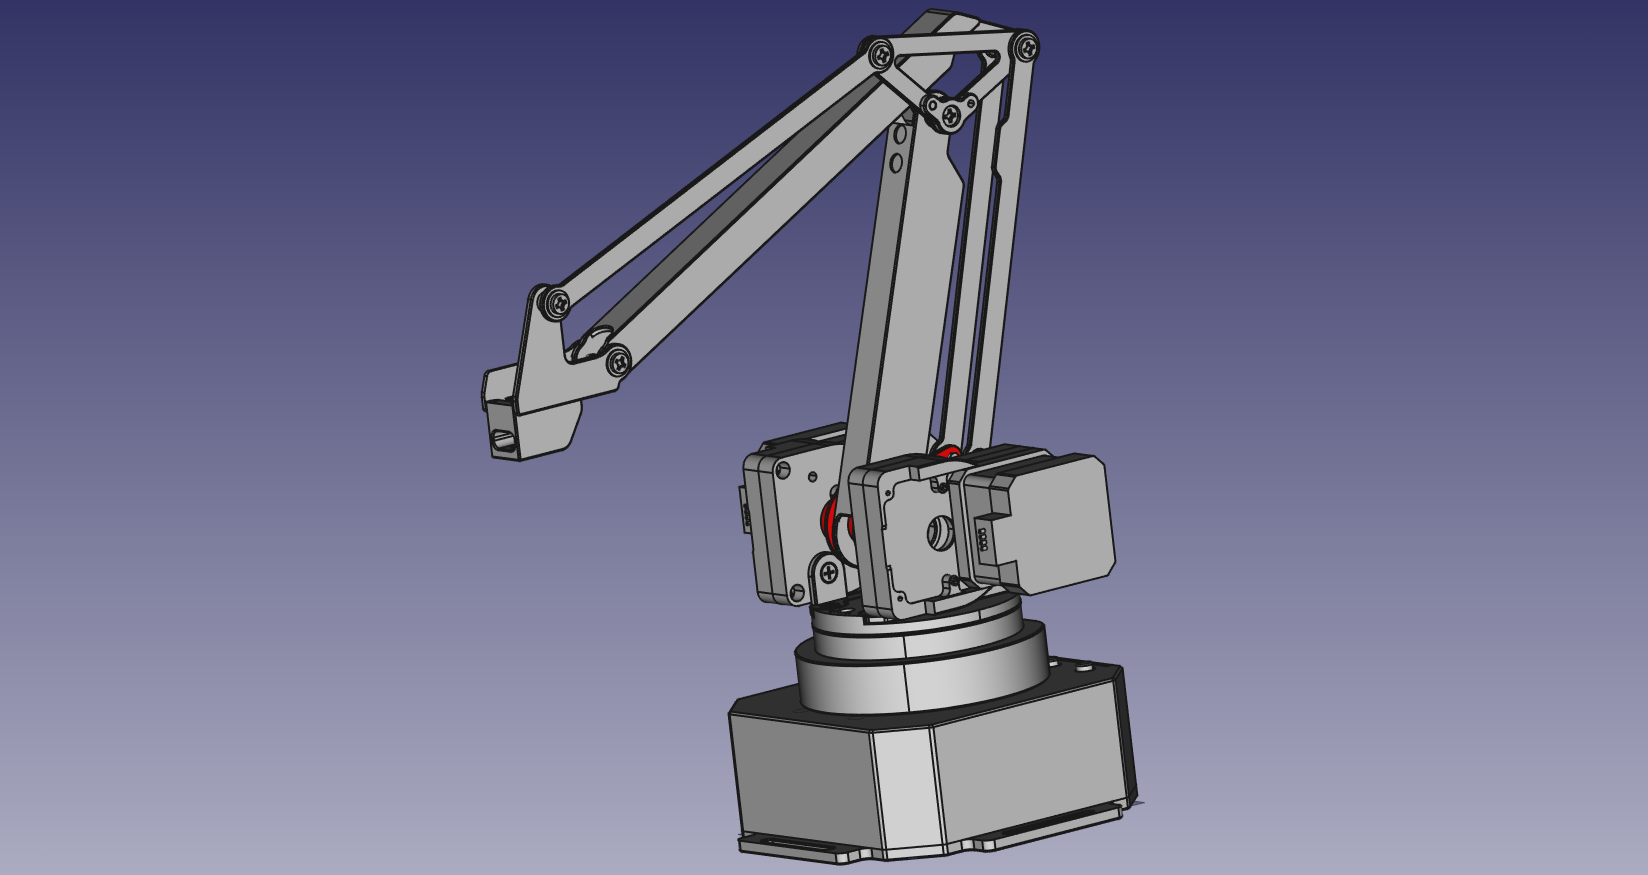
\includegraphics[width=.8\linewidth]{pictures/brazo_vista_3d_inicial.png}
    \caption{Concepto inicial del brazo robótico.}
    \label{fig:manipulador_inicial}
\end{figure}

Las herramientas que han sido empleadas para visualizar y modificar el modelo y posteriormente imprimir las piezas han sido respectivamente FreeCAD y Ultimake Cura.

\begin{figure}[H]
    \centering
    
\includegraphics[width=.45\linewidth]{pictures/freeCAD.jpg}
    \hspace{1cm}
    
\includegraphics[width=.40\linewidth]{pictures/Ultimaker_cura_logo.png}
    \caption{Logotipos de las herramientas utilizadas.}
    \label{fig:herramientas_3d}
\end{figure}

El flujo de trabajo que se ha seguido desde el modelo 3D hasta la impresión de una pieza ha sido el mostrado en la figura \ref{fig:flujo_3d}:

\begin{figure}[H]
    \centering
    \includegraphics[width=.9\linewidth]{pictures/DiagramaImpresión.jpg}
    \caption{Flujo de trabajo del desarrollo y la impresión 3D.}
    \label{fig:flujo_3d}
\end{figure}

A continuación se procederá a explicar la necesidad de remodelar ciertas piezas y los inconvenientes y contratiempos que han surgido durante el modelado y la impresión de estas.

En primer lugar se explicará la caja que alberga la placa de control y uno de los motores.

La placa de control del brazo robótico no es la misma que en el caso del $\mu$Arm de UFACTORY. Además, los motores que se han empleado en este proyecto son servomotores con carcasa y sistema de sujeción distinto que los motores paso a paso del $\mu$Arm. Debido a estos dos factores se ha tenido que diseñar nuevas partes para la base del brazo robótico..

 Mas concretamente, la necesidad de rediseñar esta parte es debida a que la base original era demasiado pequeña en superficie para permitir introducir la placa de control. Además, los servomotores no podrían haber cabido junto con la placa ya que la altura era insuficiente. Por otro lado los sistemas de sujeción presentes en la caja existente no podían ser empleados para la placa de control desarrollada en este proyecto.
 
 \begin{figure}[H]
    \centering
    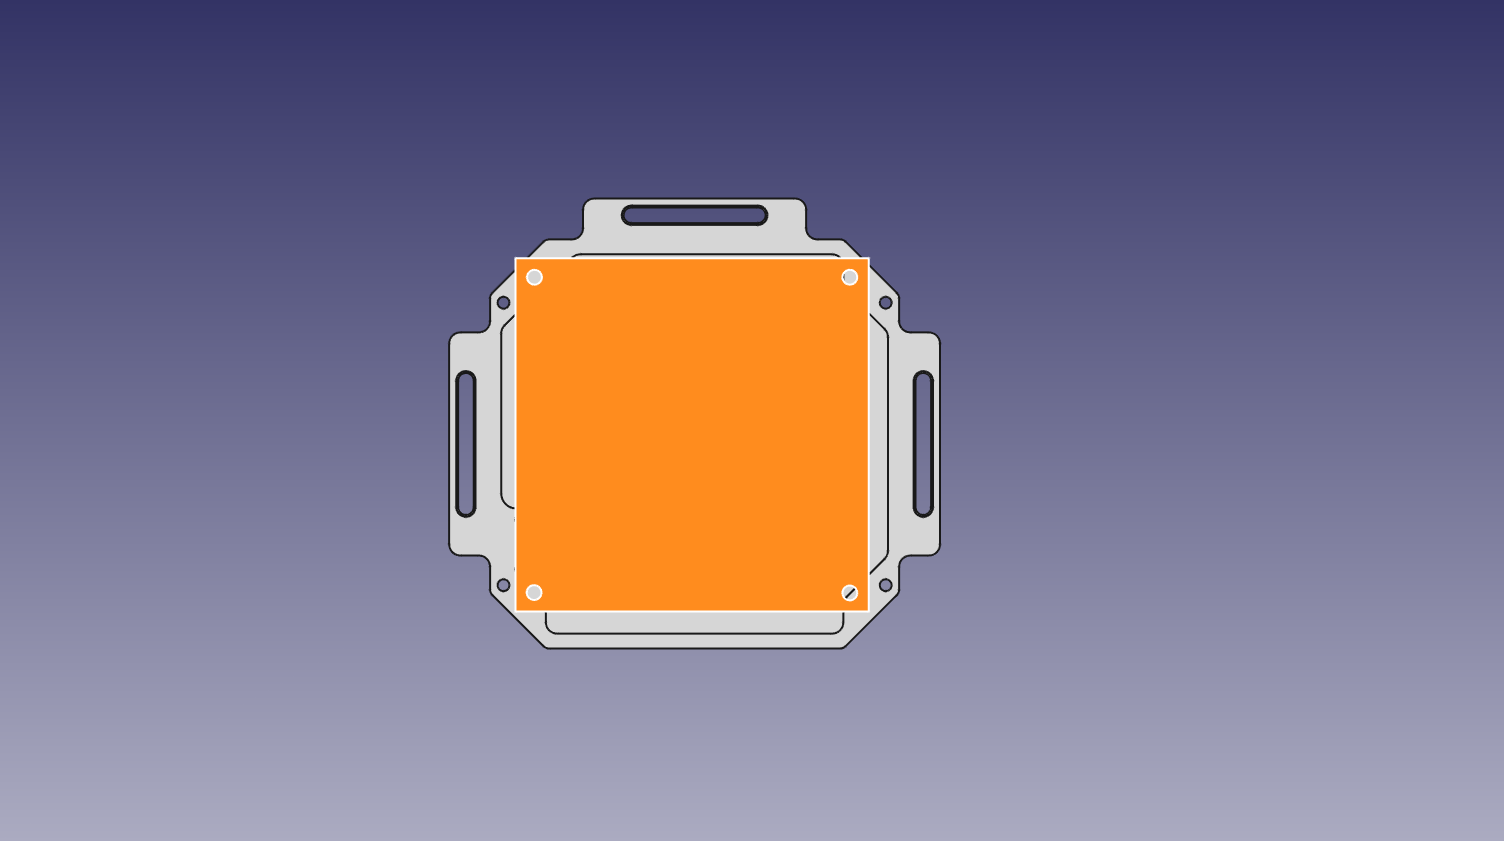
\includegraphics[width=.9\linewidth]{pictures/PlacaYBase.png}
    \caption{Proyección de la placa de control (naranja) sobre la base original del $\mu$Arm (gris)}
    \label{fig:placa_y_base_antiguas}
\end{figure}


 \begin{figure}[H]
    \centering
    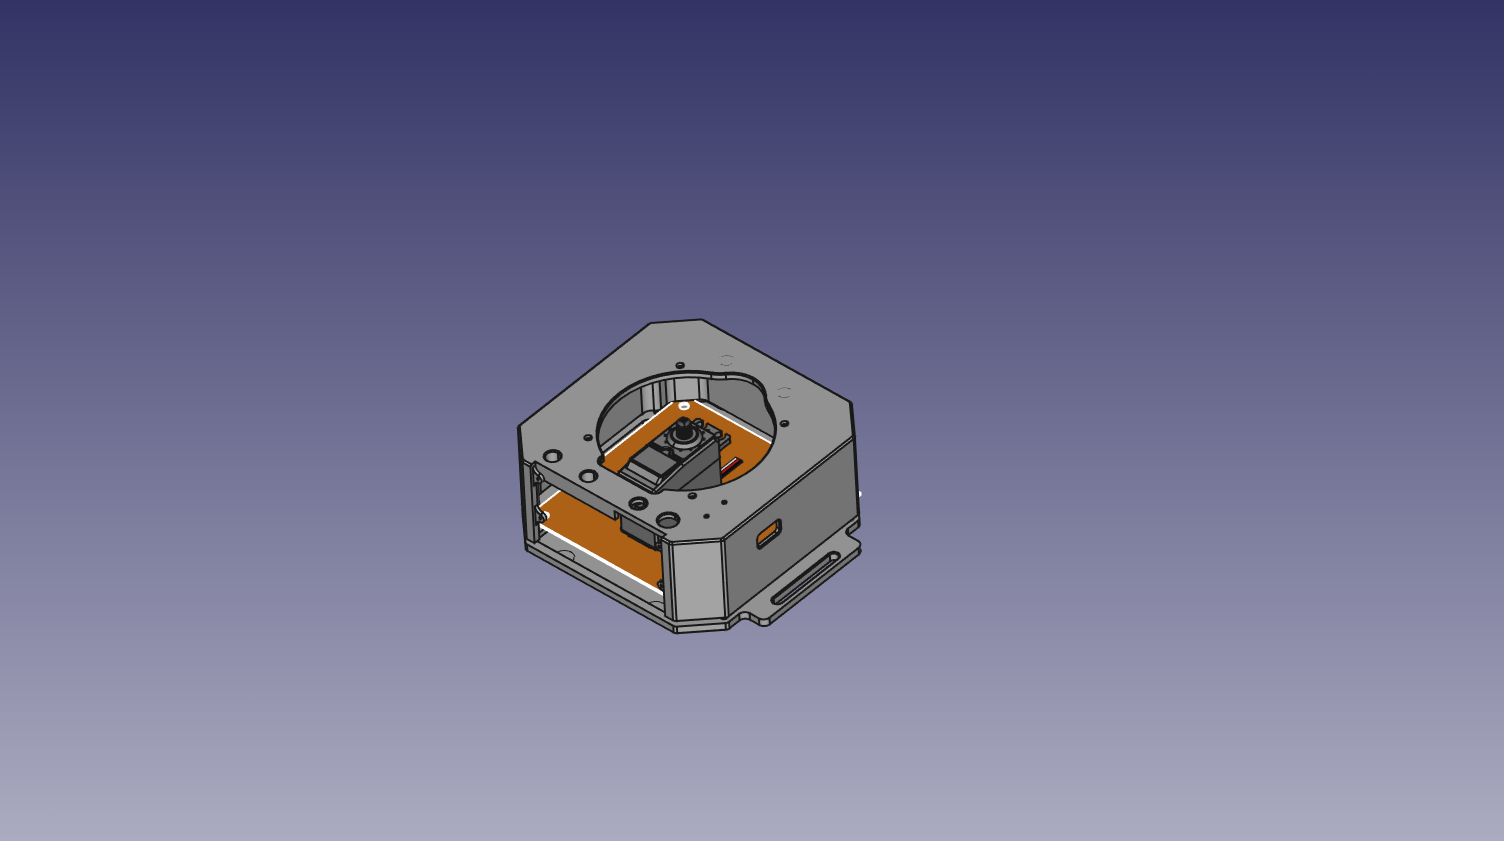
\includegraphics[width=.9\linewidth]{pictures/PlacaMotorYParedes1.png}
    \caption{Placa y motor dentro de la caja original del $\mu$Arm}
    \label{fig:placa_motor_y_paredes1}
\end{figure}

Como se observa en la figura \ref{fig:placa_motor_y_paredes1} el motor sobresale por encima de las paredes y no hay ninguna manera de sujetarlo a estas o a la base.

Para solucionar los anteriores problemas se diseña una nueva base en la que se pueda encajar la placa, además de unas paredes lo suficientemente altas para poder introducir el motor junto con la placa.

 \begin{figure}[H]
    \centering
    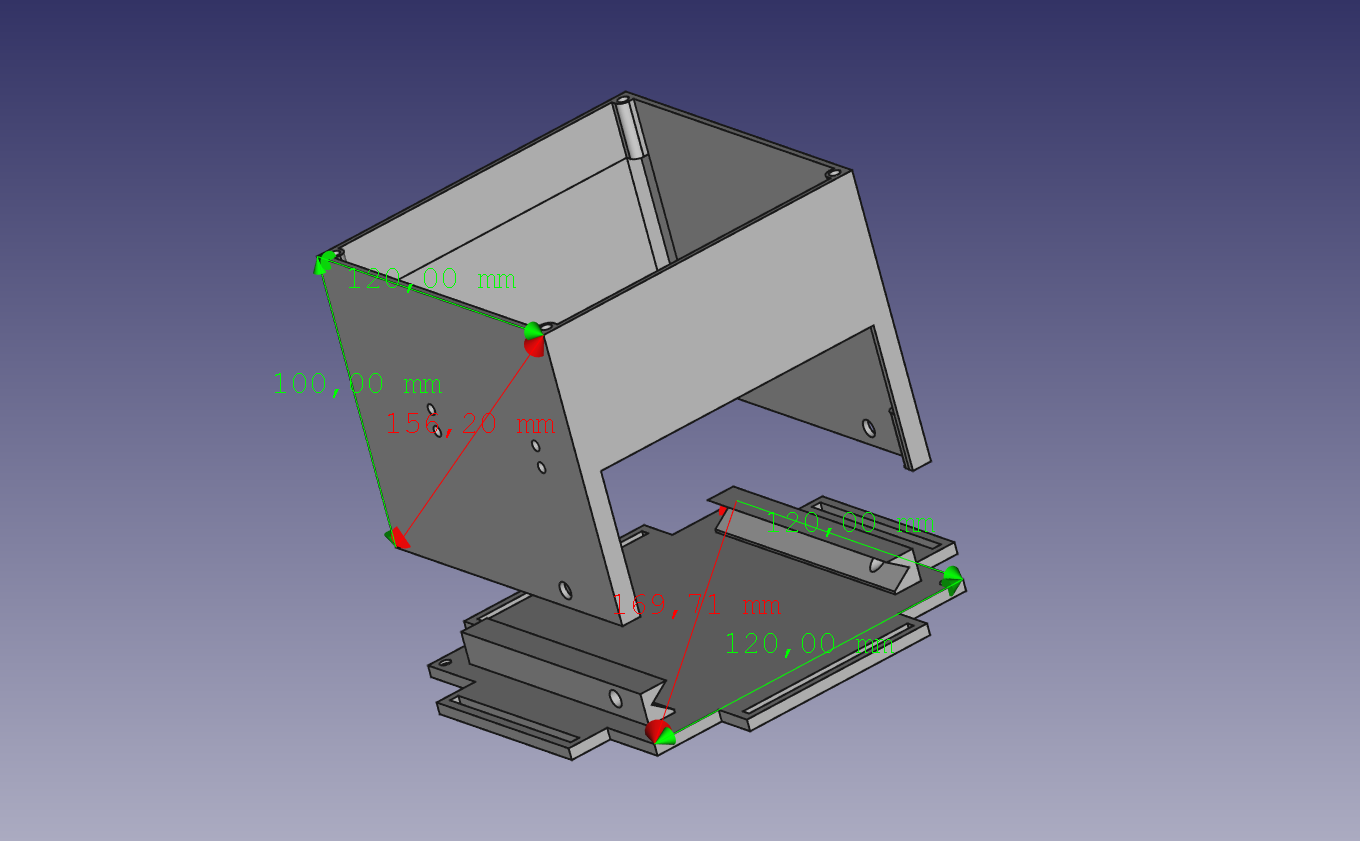
\includegraphics[width=.9\linewidth]{pictures/paredesybasenuevas.png}
    \caption{Base y paredes tras realizar las modificaciones necesarias}
    \label{fig:placa_y_paredes_nuevas}
\end{figure}

En la base se pueden observar unos carriles los cuales sirven para sujetar la placa.
Después de que la placa sea insertada en estos carriles, se asegura su posición mediante los agujeros laterales que pueden observarse en la figura \ref{fig:placa_y_paredes_nuevas}.

Cabe destacar que para poder introducir la placa en las ranuras de los carriles, se han diseñado las siguientes piezas.

 \begin{figure}[H]
    \centering
    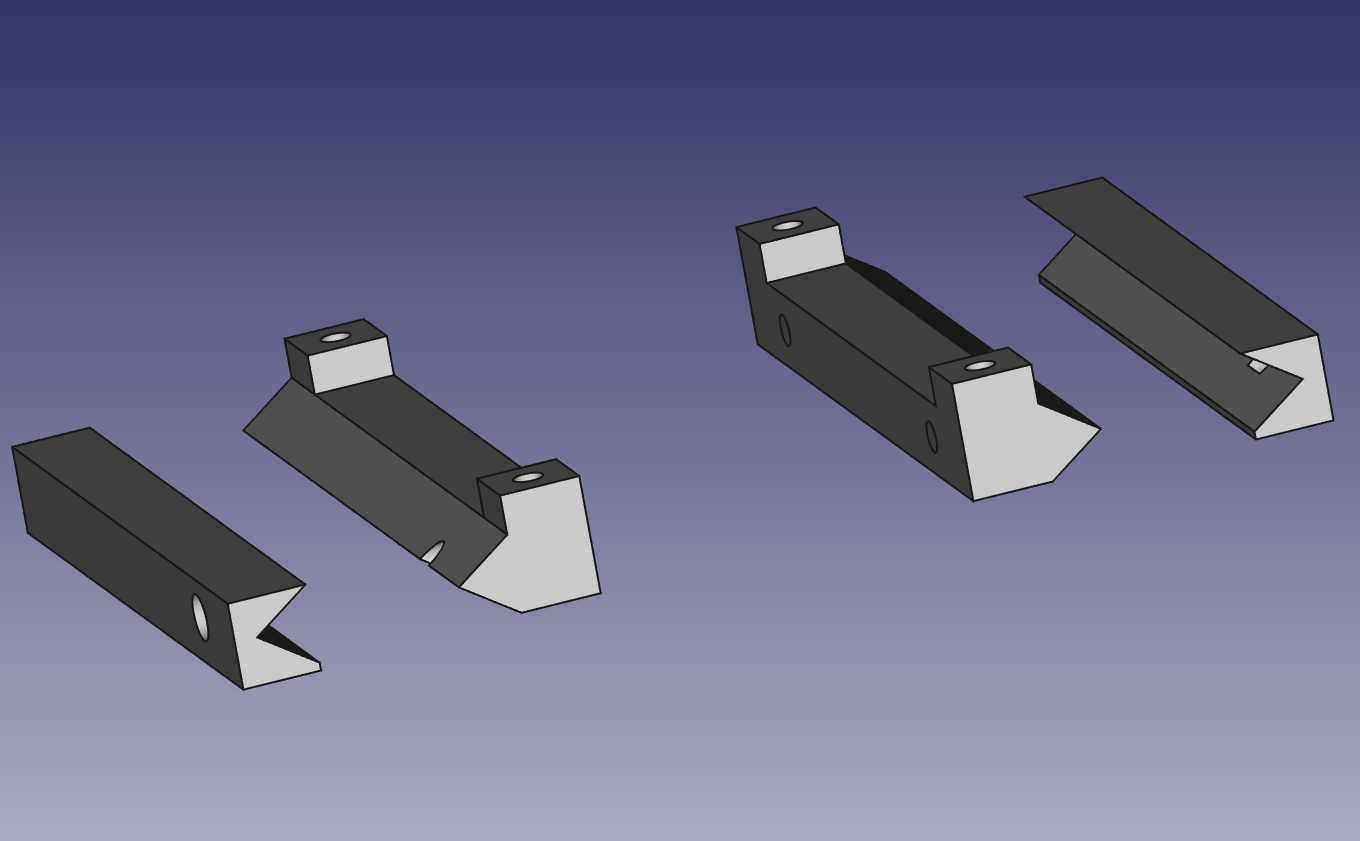
\includegraphics[width=.9\linewidth]{pictures/railes.png}
    \caption{Sistema de raíles de la placa}
    \label{fig:railes_placa}
\end{figure}


En la figura \ref{fig:railes_placa} se pueden observar los raíles que serán añadidos a la placa de control. En el exterior de la imagen se aparecen los carriles presentes en la base de la caja, donde se puede ver que al estar la placa completamente introducida en los carriles, los agujeros del carril y del raíl se posición de tal manera que se permite introducir un pasador que asegura la posición de la placa.
